% !TEX root = ../paper.tex

\section{Introduction}
Software code review is an established method regarded as a best practice in Software Engineering to achieve a sufficient quality in software project.
Its main intention is to early identify defects before integrating changes.
Nowadays, Modern Code Review (MCR)\cite{Bacchelli2013a}, less formal and lightweight code reviews have received much attention and put into software development regularly in both industrial and OSS projects.
The main benefit of MCR is that in-person meetings are not required, unlike formal inspections \cite{Fagan:1976:DCI:1661010.1661012}.
Reviewers can find defects and discuss by adding comments through a code review tool or a mailing list.
Developers will then fix their changes following those comments.

As the performance of code review straight forward to the quality of software project, many studies investigated the influencing factors in MCR\cite{Baysal2001,Mcintosh,Beller,Hamasaki2013}. However, very little research investigate that in MCR, how does a discussion for a proposed change impact to the software quality. Since most of the proposed change improvements are triggered from reviewer comments \cite{Beller}. 
It is possible that comments of reviewers can be either positively contribute the proposed changes or a discussion which is out of scope.
To determine the impact of discussion in MCR, a manual classification is required as study of Beller et. al. \cite{Beller}. As a massive amount of changes and comments in MCR history\cite{Balachandran2013,Thongtanunam2014}, it is painstaking and time consuming to classify data sets to perform quantitative analysis. Moreover, the comments in MCR is unstructured natural text unlike a checklist in the formal inspection. 
%\pick{Need some connection. Says that Massive amount of commits and comment it would be expensive to manually identify. It's natural language }
\begin{figure}[!t]
\centering
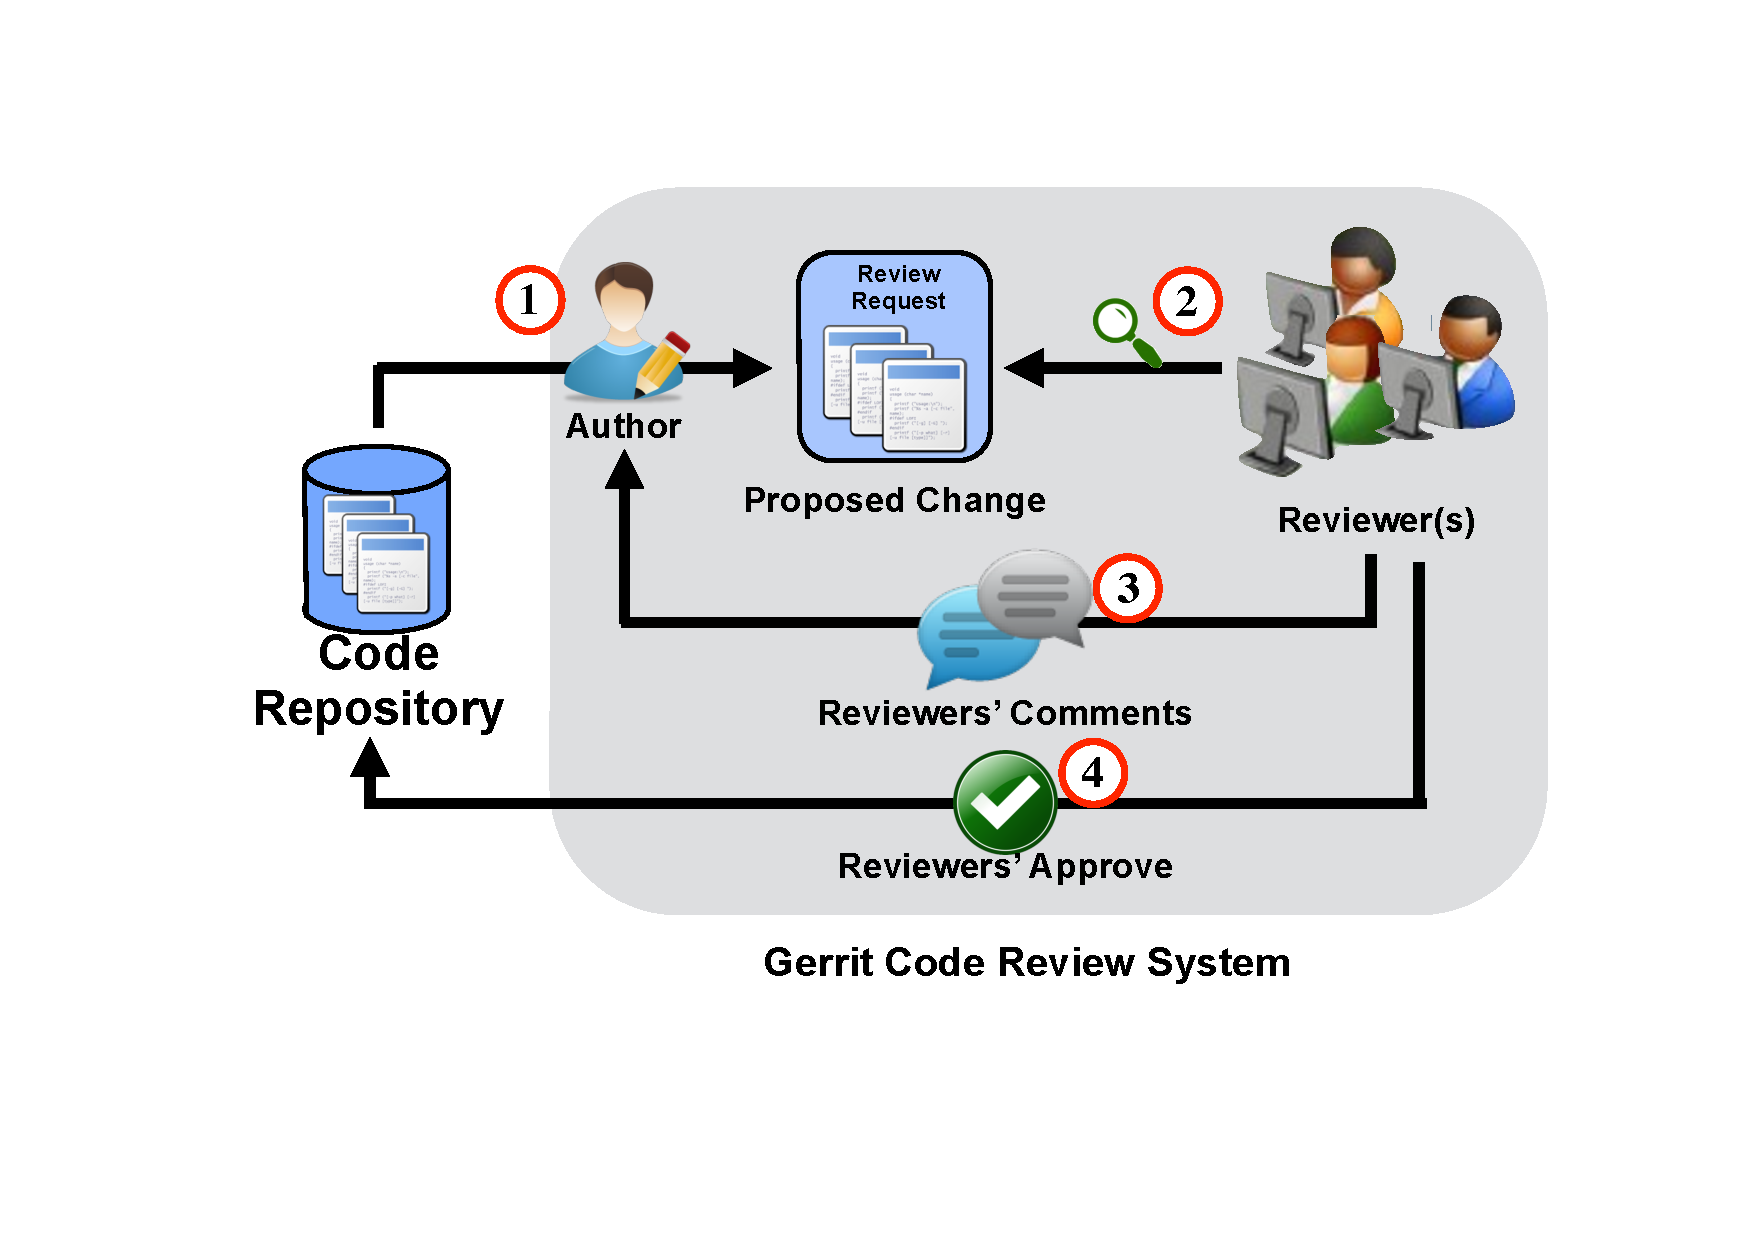
\includegraphics[scale=0.35, trim= 100 110 50 80, clip=true]{review_process}
\caption{An simplified version of MCR Process based on Gerrit system}
\label{fig:process}
\end{figure}

In this paper, we present an approach to automatically classify the usefulness of comments. We define that the usefulness is a comment that contribute to improve the proposed changes. In our approach, we analyze the similarity between commit message of the proposed changes and their comments. Our key idea is that useful comments are likely to contain similar topic as the proposed changes. To do so, we use text mining techniques, Vector Space Model (VSM) to calculate similarity and use euclidian distance to calculate dissimilarity. 
We create our predictive model by estimating a set of similarity and dissimilarity values that best discriminate between a useful and useless comments using the prediction evaluations: Precision, Recall and F-measure.

For our case study, we used a review history of Gerrit\footnote{https://code.google.com/p/gerrit/} system which is tool for supporting MCR process. Our case studied project is Qt\footnote{http://qt-project.org/}, a open source project of a cross-platform application and UI framework supported by Digia corporation. To validate our approach, we manually classify the usefulness for 320 comments and measure its accuracy. We also used our predictive model for the all set of comments to preliminary estimate quality of reviews. According to this, we address the following two research questions:

\noindent \textbf{RQ1:} Can we identify useful and useless discussions in code review?\\
\noindent \textbf{RQ2:} Do code reviewers intensively discuss on the proposed changes?\\
\noindent \textbf{RQ3:} Is this a cost-efficient way to identify useful and useless comments?

\noindent The main contribution of this paper are:
\begin{itemize}
\item We propose an approach to mine natural text of comments in code reviews and classify their usefulness.
\item The experimental results show that our approach can classify comments with XX of F-measure.
\item We found that XX\% of comments for each review are classified as useful comments, while XX \% of comments are classified as useless comments.
\end{itemize} 
%Software Inspection is basically composed of a three-step procedure: preparation, inspection meeting, and repair.

